% a mashup of hipstercv, friggeri and twenty cv
% https://www.latextemplates.com/template/twenty-seconds-resumecv
% https://www.latextemplates.com/template/friggeri-resume-cv

\documentclass[pastel]{simplehipstercv}
% available options are: darkhipster, lighthipster, pastel, allblack, grey, verylight, withoutsidebar
% withoutsidebar
\usepackage[utf8]{inputenc}
\usepackage[default]{raleway}
\usepackage[margin=1cm,a4paper]{geometry}
\usepackage[ngerman]{babel}

%------------------------------------------------------------------ Variablen

\newlength{\rightcolwidth}
\newlength{\leftcolwidth}
\setlength{\leftcolwidth}{0.23\textwidth}
\setlength{\rightcolwidth}{0.75\textwidth}

%------------------------------------------------------------------
\title{New Simple CV}
\author{\LaTeX{} Ninja}
\date{June 2019}

\pagestyle{empty}
\begin{document}


\thispagestyle{empty}
%-------------------------------------------------------------

\section*{Start}

\simpleheader{headercolour}{Samuel Weber}{Pinnock}{Physiker}{white}



%------------------------------------------------

% this has to be here so the paracols starts..
\subsection*{}
\vspace{4em}

\setlength{\columnsep}{1.5cm}
\columnratio{0.23}[0.75]
\begin{paracol}{2}
\hbadness5000
%\backgroundcolor{c[1]}[rgb]{1,1,0.8} % cream yellow for column-1 %\backgroundcolor{g}[rgb]{0.8,1,1} % \backgroundcolor{l}[rgb]{0,0,0.7} % dark blue for left margin

\paracolbackgroundoptions

% 0.9,0.9,0.9 -- 0.8,0.8,0.8


\footnotesize
{\setasidefontcolour
\flushright
\begin{center}
    \begin{figure}[H]
    \centering
    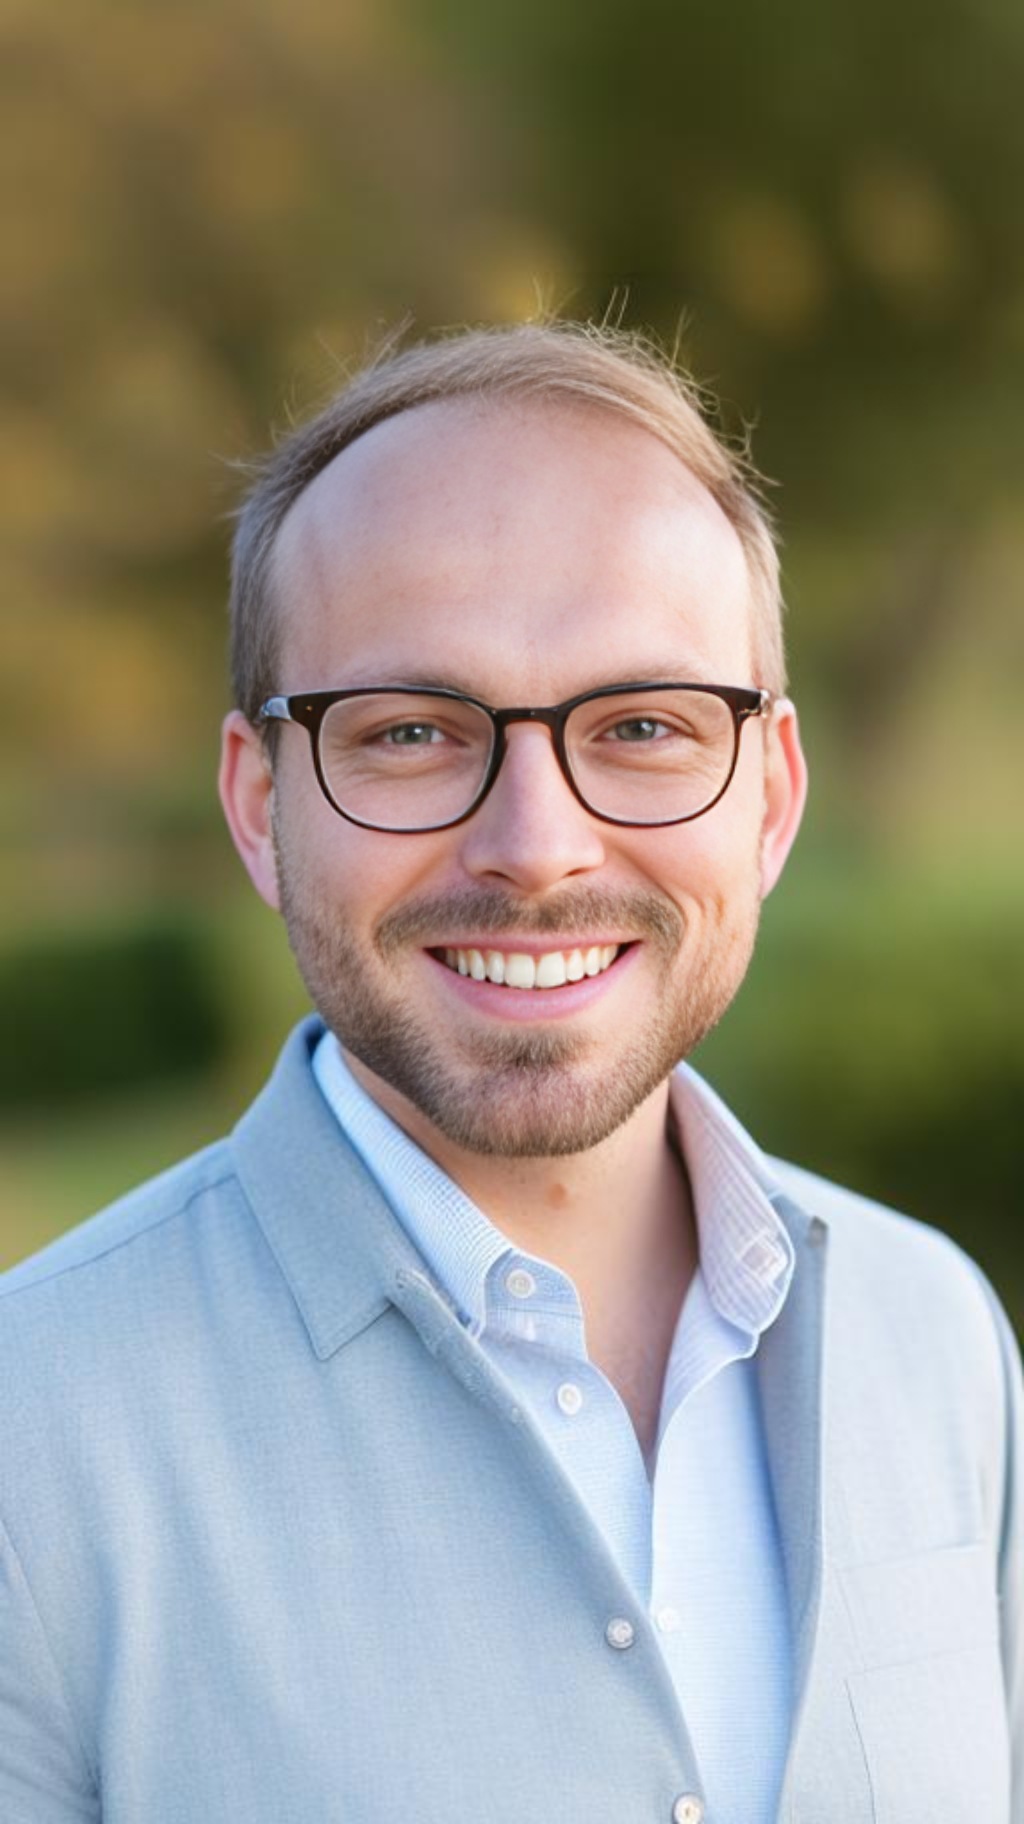
\includegraphics[height=5cm]{foto.png}
    \end{figure}
\end{center}

\bg{cvpurple}{white}{Über mich}\\[0.5em]

{\footnotesize
Mit 18 Jahren bin ich nach
Deutschland ausgewandert.
Nachdem ich die deutsche
Sprache erlernt hatte, zog ich
nach Stuttgart, um Physik zu
studieren. Im Laufe meines
Studiums konzentrierte ich
mich insbesondere auf die
Fachgebiete der
Optik, Festkörperphysik und
Atomphysik. Durch meine
akademische Laufbahn lernte
ich ein breites Spektrum an
Messmethoden und
Auswertungsverfahren kennen
und es fasziniert mich,
Messabläufe zu optimieren
und zu automatisieren,
wodurch ich meine Fähigkeiten
in der Programmierung
einsetzen kann. Präzision und
Organisation sind für mich
dabei von zentraler
Bedeutung.}
\bigskip

\bg{cvpurple}{white}{Kontakt}\\[0.5em]
{\footnotesize 
\icon{\faEnvelopeO}{cvpurple}{}pinnock.samuel@gmail.com  
\icon{\faPhone}{cvpurple}{}+49 176 8703 1622\\
\icon{\faMapMarker}{cvpurple}{}Bismarckstr. 16, \\ 73614 Schorndorf \\
Geboren: 11.09.1995 \\
Nationalität: Deutsch} 

\bigskip

\bg{cvpurple}{white}{Fachliche Schwerpunkte} \\[0.5em]

~•~ Optik ~•~ Festkörperphysik ~•~ Atomphysik 

\bigskip



\bigskip

\bg{cvpurple}{white}{Kompetenzen}\\[0.5em]
~•~ Detailorientiert ~•~ Teamfähig ~•~ Gewissenhaft
\bigskip

\bg{cvpurple}{white}{Interessen}\\[0.5em]

~•~ Ausdauertraining ~•~ Gitarre ~•~ App-Entwickler

\vspace{4em}

%\infobubble{\faAt}{cvgreen}{white}{jack@sparrow.org}
%\infobubble{\faTwitter}{cvgreen}{white}{@sparrow}
%\infobubble{\faFacebook}{cvgreen}{white}{Samuel Weber Pinnock}
%\infobubble{\faGithub}{cvgreen}{white}{sparrow}

\phantom{turn the page}

\phantom{turn the page}
}
%-----------------------------------------------------------
\switchcolumn

\small
\section*{Kurzes Resumé}

\begin{tabular}{r| p{0.5\textwidth} c}
    \cvevent{2023 - bis heute}{Produktionsingenieur Optics / Laser in der EUV}{Trumpf Lasersystems for Semiconductor Manufacturing SE + Co. KG}{Ditzingen}{
        \begin{itemize}
            \item Ich entwickle Qualifizierungssoftware via Python zur Automatisierung von baugruppenspezifische Prozesse.
            \item Ich optimiere die Montage wichtiger Produkte für EUV-Lasersysteme.
            \item Ich validiere und setze komplexe optische Qualifikationen EUV-relevanter Produkte im Bereich der Optik und Interferometrie um.
            \item Ich konzipiere und implementiere langfristige Fehlerabstellungsmaßnahmen.
            \item Ich vertrete produktsspezifischen Interessen der Produktion und fungiere als Schnittstelle zwischen den Bereichen Montage, Entwicklung, und Qualitätssicherung.
        \end{itemize} 
        }{}\\
 
\end{tabular}
\vspace{3em}

\begin{minipage}[t]{0.4\rightcolwidth}
\section*{Abschlüsse}
\begin{tabular}{r p{0.6\textwidth} c}
    \cvdegree{2019 -- 2022}{Physikstudium}{M.Sc. (1,4)}{Universität Stuttgart \color{headerblue}}{}{} \\
    \cvdegree{2016 -- 2019}{Physikstudium}{B.Sc.}{Universität Stuttgart \color{headerblue}}{}{} \\    
\end{tabular}
\section*{Sprachen}
\begin{tabular}{l | ll}
\textbf{Englisch} & C2 & {\phantom{x}\footnotesize Muttersprache} \\
\textbf{Deutsch} & C2 & \pictofraction{\faCircle}{cvpurple}{4}{black!30}{1}{\tiny} \\
\end{tabular}
\bigskip
\end{minipage}\hfill
\begin{minipage}[t]{0.4\rightcolwidth}
\section*{EDV-Kenntnisse}
\begin{tabular}{r @{\hspace{0.5em}}l}
     \bg{skilllabelcolour}{iconcolour}{Python} &  \barrule{0.55}{0.5em}{cvgreen}\\
     \bg{skilllabelcolour}{iconcolour}{Matlab} & \barrule{0.42}{0.5em}{cvpurple} \\
     \bg{skilllabelcolour}{iconcolour}{UNIX} & \barrule{0.4}{0.5em}{cvpurple} \\
     \bg{skilllabelcolour}{iconcolour}{C++} & \barrule{0.25}{0.5em}{cvpurple} \\
     \bg{skilllabelcolour}{iconcolour}{MS-Office} & \barrule{0.35}{0.5em}{cvpurple} \\
     \bg{skilllabelcolour}{iconcolour}{Zemax} & \barrule{0.2}{0.5em}{cvpurple} \\
     \bg{skilllabelcolour}{iconcolour}{javascript} & \barrule{0.1}{0.5em}{cvpurple} \\
    \end{tabular}
\end{minipage}

\section*{Messtechnik}
\begin{tabular}{r @{\hspace{0.5em}}l}
     \bg{skilllabelcolour}{iconcolour}{THz-Spektroskopie} &  \barrule{0.35}{0.5em}{cvpurple}\\
     \bg{skilllabelcolour}{iconcolour}{FTIR-Spektroskopie} & \barrule{0.3}{0.5em}{cvpurple} \\
     \bg{skilllabelcolour}{iconcolour}{Interferometrie} & \barrule{0.35}{0.5em}{cvgreen} \\
     \bg{skilllabelcolour}{iconcolour}{Umgang mit hohen Magnetfeldern} & \barrule{0.35}{0.5em}{cvpurple} \\
     \bg{skilllabelcolour}{iconcolour}{Umgang mit kryogenen Flüssigkeiten} & \barrule{0.35}{0.5em}{cvpurple} \\
     \bg{skilllabelcolour}{iconcolour}{Photolumineszenzspektroskopie} & \barrule{0.25}{0.5em}{cvpurple} \\
     \bg{skilllabelcolour}{iconcolour}{REM/AFM} & \barrule{0.15}{0.5em}{cvpurple} \\
     \bg{skilllabelcolour}{iconcolour}{Ellipsometrie} & \barrule{0.1}{0.5em}{cvpurple} \\
\end{tabular}

%\vspace{1cm}

\section*{Curriculum}
\begin{tabular}{r| p{0.5\textwidth} c}
    \cvevent{2022 -- 2023}{Physikstudium}{PhD}{Universität Stuttgart}{Charakterisierung exotischer Materialien mittels spektroskopischen Messungen mit Infrarot- und THz-Strahlung. Beaufsichtigung des THz-Labors am 1. Physikalischen Institut. Einarbeitung der Studenten in der Spektroskopie mit hohen Magnetfeldern und die Handhabung mit kryogenen Flüssigkeiten.}{} \\
    \cvevent{2019 -- 2022}{Physikstudium}{M.Sc. (1,4)}{Universität Stuttgart}{Schwerpunkt: Optik. Masterarbeit: Aufbau einer neuen Forschungsrichtung für das Institut im Bereich der THz-Vortexstrahlen. Entwicklung und Aufbau eines Interferometers für die Detektion und Qualifizierung von Vortexstrahlen. Entwicklung und Implementierung von 3D-gedruckten Optiken für THz-Strahlung.}{} \\
    \cvevent{2016 -- 2019}{Physikstudium}{B.Sc.}{Universität Stuttgart}{Schwerpunkt: Atomphysik. Bachelorarbeit: Entwicklung eines Absorptionsabbildungssystems mit infraroten Lasern für ein Ionenmikroskop, sowie die Automatisierung des Abbildungssystems mittels C++.}{} \\
    \cvevent{2014 -- 2015}{Sprachschule}{TestDaF-Prüfung}{did deutsch-institut Berlin}{Erwerb von Sprachkenntnissen in der deutschen Sprache bis C1-Niveau.}{} \\
    \cvevent{2010 -- 2014}{Highschool}{Highschool diploma}{Cherry Creek Highschool, Colorado USA}{Highschool-Abschluss mit Auszeichnung: \textit{Academic High Honors}}{} \\
\end{tabular}

\vspace{1cm}

\section*{Vorträge}
\begin{tabular}{>{\footnotesize\bfseries}r >{\footnotesize}p{0.5\textwidth}}
    März 2023 & ''Generation of THz vortex beams and interferometric determination of their topological charge,'' Frühjahrstagung der Deutschen Physikalischen Gesellschaft (DPG) Dresden, Deutschland\\\\
    Nov. 2022 & ``Incomplete screening of Ge cyclotron resonance in ordinary Voigt geometry'', \emph{Laboratoire de Physique des Solides CNRS} Paris-Saclay, Frankreich.\\\\
    Mai 2022 & ``THz vortex beams and Landau level transitions for demultiplexed orbital angular momentum detection'', Fraunhofer ITWM Kaiserslautern, Deutschland.\\\\
    Juli 2020 & ''Die Physik niederdimensionaler Strukturen'', IHFG Universität Stuttgart, Stuttgart, Deutschland. 
\end{tabular}
\vspace{1cm}

\section*{Veröffentlichungen}
\begin{tabular}{>{\footnotesize\bfseries}r >{\footnotesize}p{0.5\textwidth}}
    Jan. 2023 & S. W. Pinnock, et al., "Generation of THz Vortex Beams and Interferometric Determination of Their Topological Charge," IEEE Trans Terahertz Sci Technol IEEE T THZ SCI TECHN 2023, doi: 10.1109/TTHZ.2022.3221369. \\
\end{tabular}



\vspace{3.85cm}

%----------------------------------------------------------------------------------------
%	FINAL FOOTER
%----------------------------------------------------------------------------------------
\setlength{\parindent}{0pt}
\begin{minipage}[t]{\rightcolwidth}
\begin{center}\fontfamily{\sfdefault}\selectfont \color{black!70}
{\small Samuel W. Pinnock \icon{\faEnvelopeO}{cvpurple}{} pinnock.samuel@gmail.com \icon{\faMapMarker}{cvpurple}{} Stuttgart \icon{\faPhone}{cvpurple}{} +49 176 87031622
}
\end{center}
\end{minipage}

\end{paracol}

\end{document}
